\documentclass[11pt,a4paper]{article}

% ============================================================
% Stage 1 Specialist Mathematics investigation
% Main body: maximum 8 pages.
% AI disclosure, References and Appendices are outside the 8 pages.
% ============================================================
\usepackage[a4paper,left=1.5cm,right=1.5cm,top=1.9cm,bottom=1.9cm]{geometry}
\usepackage{amsmath,amssymb,amsthm,mathtools}
\usepackage{booktabs,array}
\usepackage{enumitem}
\usepackage{fancyhdr}
\usepackage{microtype}
\usepackage{listings}
\usepackage[T1]{fontenc}
\usepackage{lmodern}
\usepackage[font=small,labelfont=bf,skip=3pt]{caption}
\usepackage{hyperref}
\usepackage{xcolor}
\usepackage{tcolorbox}
\usepackage{graphicx}

\setlength{\parindent}{0pt}
\setlength{\parskip}{0.35em}
\setlength{\emergencystretch}{2em}

\setlist[itemize]{leftmargin=1.55em,itemsep=0.12em,topsep=0.1em}
\setlist[enumerate]{leftmargin=1.75em,itemsep=0.12em,topsep=0.1em}

\pagestyle{fancy}
\fancyhf{}
\lhead{Stage 1 Specialist Mathematics}
\rhead{Encryption using Matrices}
\cfoot{Page \thepage}
\setlength{\headheight}{14pt}

\definecolor{keyblue}{RGB}{25,65,105}
\tcbset{
    colback=gray!4,
    colframe=keyblue!55!black,
    boxrule=0.45pt,
    arc=2pt,
    left=5pt, right=5pt, top=2pt, bottom=2pt,
    before skip=3pt, after skip=3pt
}

\hypersetup{colorlinks=true, linkcolor=black, urlcolor=blue, citecolor=black}

\lstset{
    language=Python,
    basicstyle=\ttfamily\scriptsize,
    columns=fullflexible,
    keepspaces=true,
    frame=single,
    breaklines=true,
    showstringspaces=false,
    aboveskip=0.4em,
    belowskip=0.4em
}

% Compact display equations
\setlength{\abovedisplayskip}{3pt plus 1pt minus 1pt}
\setlength{\belowdisplayskip}{3pt plus 1pt minus 1pt}
\setlength{\abovedisplayshortskip}{1pt plus 1pt}
\setlength{\belowdisplayshortskip}{2pt plus 1pt}
\renewcommand{\arraystretch}{1.05}

% Notation
\newcommand{\vect}[1]{\begin{pmatrix}#1\end{pmatrix}}
\newcommand{\smat}[1]{\left(\begin{smallmatrix}#1\end{smallmatrix}\right)}
\newcommand{\x}{\mathbf{x}}   % plaintext block (column vector)
\newcommand{\y}{\mathbf{y}}   % ciphertext block (column vector)
\newcommand{\adj}{\operatorname{adj}}
% Evidence that still has to be supplied by the author (shown in red)
\newcommand{\todo}[1]{\textcolor{red}{\textbf{[TO ADD: #1]}}}

\theoremstyle{plain}
\newtheorem{theorem}{Theorem}
\theoremstyle{definition}
\newtheorem*{notation}{Notation}

\begin{document}

\begin{center}
    {\Large\textbf{Encryption Using Matrices: Testing and Improving Hill Cipher Keys}}\\[0.2em]
    {\large Jeremy Li}\\[0.1em]
    Stage 1 Specialist Mathematics --- Semester 2, 2026
\end{center}

% ============================================================
\section{Introduction}

The Hill cipher is a classical method of encryption. It was described by Lester S.\ Hill in 1929 [2, 3]. Instead of replacing one letter at a time, it changes a block of letters into a new block by matrix multiplication. All calculations are done modulo $26$, so every result can be turned back into a letter. This makes the cipher a good context for studying matrices, determinants, modular arithmetic and inverses together.

This investigation uses the letter-number convention of the task, $\text{A}\mapsto1,\ \text{B}\mapsto2,\ \ldots,\ \text{Y}\mapsto25,\ \text{Z}\mapsto0$ [1]. It is guided by three questions.
\begin{enumerate}
\item How can a $2\times2$ matrix encrypt and decrypt a message, and what makes the process reversible?
\item Which matrices are valid keys, and why does the choice of modulus matter?
\item How reasonable is the model as a way to protect a message, and what are its limitations?
\end{enumerate}

The main case study is our submitted Matrix Quiz / Encryption Activity, where the plaintext is $\text{ILOVESENRENBANKA}$ and the key matrix is $K=\smat{9&4\\2&7}$. A second message, ``Genshin Impact is the most fun game'', tests the method on a longer message that needs padding. We also decrypted a ciphertext written by another student. The report includes worked calculations and calculator checks. GPT generated and revised the Python code, then ran the program checks and tests (Section~\ref{sec:tech}). The author used GPT explanations to understand the output, then used the coding results to develop the investigation.


% ============================================================
\section{Mathematical Background}

\subsection{Modular arithmetic}

For integers $a$ and $b$ and a positive integer $m$, we write $a\equiv b\pmod m$ when $a-b$ is divisible by $m$. For example, $27\equiv1\pmod{26}$ and $-1\equiv25\pmod{26}$. Every integer is congruent modulo $26$ to exactly one of $0,1,\ldots,25$, which is the remainder after division by $26$. This is why modulus $26$ is used: a result such as $129$ has no matching letter, but $129\equiv25\pmod{26}$ does.

The task uses $\text{Z}\mapsto0$ so that the $26$ letters match the $26$ remainders, and the GPT-generated Python program uses the same convention. Writing $\text{Z}\mapsto26$ is equivalent because $26\equiv0\pmod{26}$, provided it is applied consistently.

\subsection{Modular inverses}

An integer $b$ is a \emph{modular multiplicative inverse} of $a$ modulo $m$ if $ab\equiv1\pmod m$. For example, $5(21)=105=4(26)+1$, so $5^{-1}\equiv21\pmod{26}$. Inverses are needed because decryption must ``undo'' a multiplication, and in modular arithmetic division means multiplying by an inverse. Not every number has one: $2$ has no inverse modulo $26$, because $2x-26k=1$ is impossible when the left side is always even.

\begin{theorem}\label{thm:inverse}
An integer $a$ has an inverse modulo $m$ if and only if $\gcd(a,m)=1$.
\end{theorem}
\begin{proof}
If $\gcd(a,m)=1$, Bézout's identity [6, 7] gives integers $s,t$ with $as+mt=1$, so $as\equiv1\pmod m$. Conversely, if $ab\equiv1\pmod m$, then $ab-km=1$ for some integer $k$. Any common divisor of $a$ and $m$ divides $ab-km=1$, so $\gcd(a,m)=1$.
\end{proof}

Since $26=2\times13$, a number has an inverse modulo $26$ exactly when it is odd and not a multiple of $13$. Table~\ref{tab:inverses} lists the $12$ numbers that qualify. Only $12$ of the $26$ remainders can be used, which already suggests that valid keys will be limited.

\begin{table}[ht]
\centering
\small
\caption{Numbers with an inverse modulo $26$ (each pair satisfies $a\,a^{-1}\equiv1$).}
\label{tab:inverses}
\setlength{\tabcolsep}{5pt}
\begin{tabular}{l *{12}{r}}
\toprule
$a$ & 1 & 3 & 5 & 7 & 9 & 11 & 15 & 17 & 19 & 21 & 23 & 25\\
$a^{-1}$ & 1 & 9 & 21 & 15 & 3 & 19 & 7 & 23 & 11 & 5 & 17 & 25\\
\bottomrule
\end{tabular}
\end{table}

\subsection{The Hill cipher model}

The message is written in capital letters with spaces and punctuation removed. If the number of letters is odd, the letter X is added at the end, so that the message divides into blocks of two letters [5]. Each block is written as a column vector. For example, $\text{AL}\longrightarrow\x=(1,12)^T$, where $\x=(x_1,x_2)^T$ is a plaintext block. A ciphertext block is $\y=(y_1,y_2)^T$. The key is a matrix $K=\smat{a&b\\c&d}$ with integer entries. Encryption and decryption are [2, 5]
\[
\y\equiv K\x\pmod{26},
\qquad
\x\equiv K^{-1}\y\pmod{26},
\]
where $K^{-1}$ is the inverse of $K$ modulo $26$, meaning $K^{-1}K\equiv KK^{-1}\equiv I\pmod{26}$. (The task sheet writes this as $K^{-1}_{26}$.) Decryption works because $K^{-1}\y\equiv K^{-1}(K\x)\equiv(K^{-1}K)\x\equiv\x$. In full,
\[
y_1\equiv ax_1+bx_2,\qquad y_2\equiv cx_1+dx_2\pmod{26}.
\]
Each ciphertext value usually depends on both letters of the block (Section~\ref{sec:main} explains an exception), so the cipher is not a letter-by-letter substitution.

\subsection{Determinants and the inverse key}

Let $\Delta=\det K=ad-bc$ and $\adj K=\smat{d&-b\\-c&a}$. Direct multiplication gives
\[
K\,\adj K=\adj K\,K=\vect{ad-bc&0\\0&ad-bc}=\Delta I.
\]
If $\Delta$ has an inverse modulo $26$, then $K^{-1}\equiv\Delta^{-1}\adj K\pmod{26}$ [2, 5, 8]. By Theorem~\ref{thm:inverse}, this requires $\gcd(\Delta,26)=1$, so $\Delta$ must be odd and not a multiple of $13$. The value $\Delta$ can be negative or large, so it is reduced modulo $26$ first. This is allowed because $\Delta$ and $\Delta\bmod 26$ differ by a multiple of $26$, so they have the same $\gcd$ with $26$. The task sheet allows real entries, but modular arithmetic needs integers, so all key entries here are integers. Section~\ref{sec:valid} proves that this condition is also necessary.

% ============================================================
\section{Main Case Study: Submitted Encryption Example}\label{sec:main}

\subsection{Testing the key and finding the inverse}

For $K=\smat{9&4\\2&7}$, the determinant is $\Delta=9(7)-4(2)=55\equiv3\pmod{26}$. Since $\gcd(3,26)=1$, the key is valid. The inverse of $3$ is $9$, because $3(9)=27\equiv1$, so
\[
K^{-1}\equiv9\vect{7&-4\\-2&9}=\vect{63&-36\\-18&81}\equiv\vect{11&16\\8&3}\pmod{26}.
\]
As a check, $K^{-1}K\equiv I\pmod{26}$.

\subsection{Encrypting the plaintext}

The plaintext has $16$ letters, so no padding is needed. It divides into eight blocks: IL, OV, ES, EN, RE, NB, AN, KA. For the first block, $\text{IL}\longrightarrow\x=(9,12)^T$ and
\[
\y=\vect{9&4\\2&7}\vect{9\\12}=\vect{129\\102}\equiv\vect{25\\24}\pmod{26},
\]
so $\text{IL}\longrightarrow\text{YX}$, because $25\mapsto\text{Y}$ and $24\mapsto\text{X}$. Table~\ref{tab:main} shows the same calculation for all eight blocks, and gives the ciphertext
\[
\boxed{\text{YXOBQMWDZSDPMVYC}}
\]
which agrees with our submitted activity.

\begin{table}[ht]
\centering
\small
\caption{Encryption and decryption of ILOVESENRENBANKA with $K=\smat{9&4\\2&7}$. Each pair $(u,v)$ stands for the column vector $(u,v)^T$.}
\label{tab:main}
\setlength{\tabcolsep}{6pt}
\begin{tabular}{l r r r l r r}
\toprule
Plain & $\x$ & $K\x$ & $\y=K\x\bmod26$ & Cipher & $K^{-1}\y$ & $K^{-1}\y\bmod26$\\
\midrule
IL & (9, 12)  & (129, 102) & (25, 24) & YX & (659, 272) & (9, 12)\\
OV & (15, 22) & (223, 184) & (15, 2)  & OB & (197, 126) & (15, 22)\\
ES & (5, 19)  & (121, 143) & (17, 13) & QM & (395, 175) & (5, 19)\\
EN & (5, 14)  & (101, 108) & (23, 4)  & WD & (317, 196) & (5, 14)\\
RE & (18, 5)  & (182, 71)  & (0, 19)  & ZS & (304, 57)  & (18, 5)\\
NB & (14, 2)  & (134, 42)  & (4, 16)  & DP & (300, 80)  & (14, 2)\\
AN & (1, 14)  & (65, 100)  & (13, 22) & MV & (495, 170) & (1, 14)\\
KA & (11, 1)  & (103, 29)  & (25, 3)  & YC & (323, 209) & (11, 1)\\
\bottomrule
\end{tabular}
\end{table}

Table~\ref{tab:main} shows three features. First, the letter E appears three times in the plaintext (ES, EN, RE), but the blocks QM, WD and ZS have no letter in common. Second, the ciphertext letters Y, M and D each appear twice, but each pair comes from different plaintext letters (the two Ys come from IL and KA). Third, the block RE gives $y_1=0$, written as Z, so the convention $\text{Z}\mapsto0$ affects the result. A plaintext letter therefore does not always give the same ciphertext letter, which is the main difference from a substitution cipher, where single-letter frequencies would reveal the plaintext [3, 8]. With only $16$ letters, however, this is a small sample and not a proof.

One correction is needed. If only the second letter of a block changes by $\delta$, then $y_1$ changes by $4\delta$ for this key. This is $0$ modulo $26$ when $\delta=13$, so $y_1$ does not change at all. For example, IL gives YX and IY gives YK, because L ($12$) and Y ($25$) differ by $13$, whereas IM gives CE. The reason is that the entry $4$ shares a factor with $26$. So the mixing within a block is strong in general, but not complete for every pair of letters.

\subsection{Decrypting the ciphertext}

Decryption uses $K^{-1}\equiv\smat{11&16\\8&3}$. For the first ciphertext block, $\text{YX}\longrightarrow\y=(25,24)^T$ and
\[
\x=\vect{11&16\\8&3}\vect{25\\24}=\vect{659\\272}\equiv\vect{9\\12}\pmod{26},
\]
so $\text{YX}\longrightarrow\text{IL}$. The last two columns of Table~\ref{tab:main} show that all eight blocks return to the original $\x$, so the plaintext ILOVESENRENBANKA is recovered exactly. Values such as $659$ and $272$ must be reduced modulo $26$ before they are changed back into letters.

\subsection{Decrypting another student's ciphertext}\label{sec:peer}

To test decryption on a message that we did not write, we decrypted a ciphertext from another student: \texttt{MKREMTBTSH}, with key $K=\smat{8&1\\9&3}$. Our answer sheet (Appendix~B) uses $\text{A}\mapsto1,\ldots,\text{Z}\mapsto26$, which agrees with the task convention because $26\equiv0$.

The determinant is $\Delta=8(3)-1(9)=15$ and $\gcd(15,26)=1$, so the key is valid. Since $15(7)=105=4(26)+1$, $15^{-1}\equiv7$ and
\[
K^{-1}\equiv7\vect{3&-1\\-9&8}=\vect{21&-7\\-63&56}\equiv\vect{21&19\\15&4}\pmod{26},
\]
with the check $KK^{-1}=\smat{183&156\\234&183}\equiv I$. For the first block, $\text{MK}\longrightarrow\y=(13,11)^T$ and $K^{-1}\y=(482,239)^T\equiv(14,5)^T$, because $482=18(26)+14$ and $239=9(26)+5$. So $\text{MK}\longrightarrow\text{NE}$. Table~\ref{tab:peer} gives all five blocks. The plaintext $\text{NEEDCOFFEE}$ is meaningful English, which is good evidence that the inverse is correct, because a wrong inverse would almost certainly give nonsense.

\begin{table}[ht]
\centering
\small
\caption{Decrypting \texttt{MKREMTBTSH} with $K^{-1}$, then re-encrypting the plaintext with $K=\smat{8&1\\9&3}$ as a check.}
\label{tab:peer}
\setlength{\tabcolsep}{5pt}
\begin{tabular}{l r r r l r r l}
\toprule
Cipher & $\y$ & $K^{-1}\y$ & mod 26 & Plain & $K\x$ & mod 26 & Cipher again\\
\midrule
MK & (13, 11) & (482, 239) & (14, 5) & NE & (117, 141) & (13, 11) & MK\\
RE & (18, 5)  & (473, 290) & (5, 4)  & ED & (44, 57)   & (18, 5)  & RE\\
MT & (13, 20) & (653, 275) & (3, 15) & CO & (39, 72)   & (13, 20) & MT\\
BT & (2, 20)  & (422, 110) & (6, 6)  & FF & (54, 72)   & (2, 20)  & BT\\
SH & (19, 8)  & (551, 317) & (5, 5)  & EE & (45, 60)   & (19, 8)  & SH\\
\bottomrule
\end{tabular}
\end{table}


% ============================================================
\section{Self-created Example: Genshin Impact}

\subsection{Preparing the message and the key}

The second message is ``Genshin Impact is the most fun game.'' After spaces and punctuation are removed, it is $\text{GENSHINIMPACTISTHEMOSTFUNGAME}$, which has $29$ letters. A $2\times2$ key needs an even number of letters, so one X is added, giving $\text{GENSHINIMPACTISTHEMOSTFUNGAMEX}$. We chose X because it is rare in English, so it is unlikely to be confused with a real letter. This is not perfect, and it is discussed in Section~\ref{sec:eval}.

The key is $K=\smat{4&1\\3&2}$. We chose it because its small entries are easy to work with by hand, and because the task sheet uses the same key for the word ALGEBRA [1]. That example gives an independent test (Section~\ref{sec:tech}). The determinant is $\Delta=4(2)-1(3)=5$ and $\gcd(5,26)=1$, so the key is valid. Since $5^{-1}\equiv21$,
\[
K^{-1}\equiv21\vect{2&-1\\-3&4}\equiv\vect{16&5\\15&6}\pmod{26},
\qquad
KK^{-1}=\vect{79&26\\78&27}\equiv I\pmod{26}.
\]

\subsection{Encryption and decryption}

The message divides into $15$ blocks. For the first block, $\text{GE}\longrightarrow(7,5)^T$ and
$K\x=(33,31)^T\equiv(7,5)^T\pmod{26}$, so GE is unchanged. For the second block, $\text{NS}\longrightarrow(14,19)^T$ and $K\x=(75,80)^T\equiv(23,2)^T$, so $\text{NS}\longrightarrow\text{WB}$. Table~\ref{tab:second} gives all blocks.

\begin{table}[ht]
\centering
\small
\caption{Plaintext and ciphertext blocks for the second message with $K=\smat{4&1\\3&2}$.}
\label{tab:second}
\setlength{\tabcolsep}{3.2pt}
\begin{tabular}{l *{15}{l}}
\toprule
Plaintext  & GE & NS & HI & NI & MP & AC & TI & ST & HE & MO & ST & FU & NG & AM & EX\\
Ciphertext & GE & WB & OP & MH & PS & GI & KZ & RS & KH & OQ & RS & SH & KD & QC & RK\\
\bottomrule
\end{tabular}
\end{table}

The ciphertext is $\text{GEWBOPMHPSGIKZRSKHOQRSSHKDQCRK}$, which has $30$ letters and matches the padded plaintext. To decrypt the second block, $K^{-1}(23,2)^T=(378,357)^T\equiv(14,19)^T$, which is NS. In the run completed by GPT, the program decrypted all $15$ blocks and returned $\text{GENSHINIMPACTISTHEMOSTFUNGAMEX}$, so the method works for a message that we created independently.

\subsection{Interpreting the unchanged block and the repeated block}

Two features of Table~\ref{tab:second} need explanation. First, GE is unchanged: it is a \emph{fixed block}, with $K\x\equiv\x$, which means $(K-I)\x\equiv\mathbf{0}\pmod{26}$. For this key, $K-I=\smat{3&1\\3&1}$ has identical rows, so the two equations reduce to $3x_1+x_2\equiv0$, and every $x_1$ has exactly one solution $x_2\equiv-3x_1$. This gives $26$ fixed blocks out of $676$, and GE is one of them because $3(7)+5=26\equiv0$. For the first key, $K-I=\smat{8&4\\2&6}$ has $\det(K-I)=40\equiv14$, and only four blocks are fixed: ZZ, ZM, MZ and MM. In fact, only ZZ is fixed when $K-I$ is invertible modulo $26$ (this follows from the test in Section~\ref{sec:valid}), and neither of our keys has that property. A fixed block is unchanged by encryption. Without knowing the key, an attacker may not know which blocks are fixed. The second key leaves more blocks unchanged than most valid keys (Appendix C).

Second, the block ST appears twice in the plaintext (blocks 8 and 11) and gives RS both times. The key is applied to every block in the same way, so equal plaintext blocks always give equal ciphertext blocks. This is a pattern that an attacker can see, and it is a limitation that is examined in Section~\ref{sec:security}.

% ============================================================

\subsection{Choosing a key with fewer fixed blocks}
The second key leaves $26$ blocks unchanged. We therefore look for a key with fewer fixed blocks. The new key must be invertible, and $K-I$ must also be invertible. The second condition ensures that $(K-I)\x\equiv\mathbf{0}$ has only the zero solution. We choose
\[
K_{\rm new}=\smat{1&1\\1&2},\qquad
\det K_{\rm new}=1,\qquad \det(K_{\rm new}-I)=-1.
\]
Both determinants are coprime to $26$. The new key is valid and fixes only ZZ. Its inverse is $\smat{2&25\\25&1}$ modulo $26$. GE now encrypts to LQ, instead of remaining GE. The number of fixed blocks falls from $26$ to $1$ out of $676$. The Python run completed by GPT confirms that encryption and decryption recover the full padded message.

This improves the chosen property, but it does not make the cipher secure. Repeated ST blocks still give the same ciphertext, MG. The known-plaintext attack also works: the columns GE and NS give a determinant of $63$, which is coprime to $26$. Their matching ciphertext blocks LQ and GZ therefore recover the new key. We have reduced the fixed-block problem, while the linear weakness remains.

\section{Technology Verification}\label{sec:tech}

GPT generated and revised the Python code and its tests. GPT ran the checks, including a run in the local VS Code terminal. The author studied the output with GPT support and used the results to investigate the mathematical questions. Modulo reductions were checked with the CalculatorSoup Modulo Calculator [10], and $\gcd$ values were calculated with a TI-84 Plus CE graphing calculator [11]. The Python program in Appendix A encrypts and decrypts messages, tests keys, finds inverses, counts valid keys, analyses fixed blocks and carries out the known-plaintext attack. The worked calculations explain the methods used. The program rejects keys with $\gcd(\Delta,26)\neq1$, finds inverses with the extended Euclidean algorithm (the computational form of Bézout's identity [6, 7]), uses bit masks so that testing all $456\,976$ matrices needs little memory, and includes unit tests (Appendix C).

GPT ran the following program checks against the worked examples and task sheet.
\begin{enumerate}
\item The inverse keys shown in the worked calculations $\smat{11&16\\8&3}$, $\smat{16&5\\15&6}$ and $\smat{21&19\\15&4}$ agree with the program output, and $K^{-1}K\equiv I$ modulo $26$ in each case.
\item All messages were encrypted and then decrypted, returning the original text each time. This tests that encryption and decryption are consistent.
\item The program encrypts ALGEBRAA with $K=\smat{4&1\\3&2}$ to give PAGEZPEE, matching the task sheet's worked example [1], which was produced independently of our work. This tests the letter-number convention, including $\text{Z}\mapsto0$.
\item The other student's ciphertext decrypts to meaningful English and re-encrypts to the original ciphertext (Section~\ref{sec:peer}).
\end{enumerate}


% ============================================================
\section{Investigation: Which Keys Are Valid?}\label{sec:valid}

\subsection{A conjecture and tests}

In both examples the determinant was relatively prime to $26$, and the key worked. This leads to a conjecture:

\begin{quote}
A $2\times2$ integer matrix $K$ is invertible modulo $26$ if and only if $\gcd(\det K,26)=1$.
\end{quote}

Here, ``invertible modulo $26$'' means that there is an integer matrix $B$ with $KB\equiv BK\equiv I\pmod{26}$. We tested the conjecture on seven matrices (Table~\ref{tab:keys}), including one with a negative determinant and others whose determinants share the factor $2$ or $13$ with $26$.

\begin{table}[ht]
\centering
\small
\caption{Tests of the determinant condition. The last column gives a non-zero block that the key sends to ZZ.}
\label{tab:keys}
\setlength{\tabcolsep}{7pt}
\begin{tabular}{l r r r l r}
\toprule
Key matrix $K$ & $\Delta$ & $\Delta\bmod26$ & $\gcd(\Delta,26)$ & Valid? & Block sent to ZZ\\
\midrule
$\smat{9&4\\2&7}$  & 55 & 3  & 1  & Yes & ---\\
$\smat{4&1\\3&2}$  & 5  & 5  & 1  & Yes & ---\\
$\smat{1&4\\2&1}$  & $-7$ & 19 & 1 & Yes & ---\\
$\smat{1&0\\0&2}$  & 2  & 2  & 2  & No  & (0, 13)\\
$\smat{3&2\\1&4}$  & 10 & 10 & 2  & No  & (0, 13)\\
$\smat{13&0\\0&1}$ & 13 & 13 & 13 & No  & (2, 0)\\
$\smat{5&2\\1&3}$  & 13 & 13 & 13 & No  & (20, 2)\\
\bottomrule
\end{tabular}
\end{table}

The last column shows what goes wrong with an invalid key. Every key sends the block ZZ to ZZ, because $K\mathbf{0}=\mathbf{0}$. An invalid key also sends a second block to ZZ; for example, $\smat{1&0\\0&2}\smat{0\\13}=\smat{0\\26}\equiv\smat{0\\0}$. A receiver who sees ZZ cannot tell which block was sent, so decryption is impossible. This idea can be used as a test, because $K(\x-\x')=K\x-K\x'$. Two blocks give the same ciphertext exactly when a non-zero block is sent to ZZ. If no such block exists, different blocks always give different ciphertexts, and since there are only finitely many blocks, every ciphertext block can be decrypted.

GPT ran the Python program to apply this test to all $26^4=456\,976$ matrices. Exactly $157\,248$ matrices send no non-zero block to ZZ, and these are exactly the matrices with $\gcd(\Delta,26)=1$ (Appendix C). This supports the conjecture strongly. This checks every matrix modulo $26$. An algebraic proof follows to explain why the rule works.

\subsection{Proof of the conjecture}

\begin{theorem}\label{thm:keys}
A $2\times2$ integer matrix $K$ is invertible modulo $26$ if and only if $\gcd(\Delta,26)=1$, where $\Delta=\det K$.
\end{theorem}
\begin{proof}
($\Leftarrow$) Suppose $\gcd(\Delta,26)=1$. By Theorem~\ref{thm:inverse}, $\Delta^{-1}$ exists modulo $26$. Let $B=\Delta^{-1}\adj K$. Since $K\adj K=\adj K\,K=\Delta I$ (Section 2.4), $KB\equiv BK\equiv I\pmod{26}$.

($\Rightarrow$) Suppose $KB\equiv I\pmod{26}$ for an integer matrix $B$. The determinant is a polynomial in the matrix entries, so congruent matrices have congruent determinants. Hence $\det(K)\det(B)=\det(KB)\equiv\det(I)=1\pmod{26}$. This means $\Delta$ has an inverse modulo $26$, so $\gcd(\Delta,26)=1$ by Theorem~\ref{thm:inverse}.
\end{proof}

This agrees with the $2\times2$ rule in [8]: a matrix is invertible modulo $26$ exactly when its determinant has an inverse. Invertibility modulo $26$ is stricter than ordinary invertibility: for real matrices $\Delta\neq0$ is enough, but modulo $26$ a determinant such as $2$ is non-zero and still not allowed, because $26=2\times13$.

\subsection{Why modulus 26? Counting valid keys}

The theorem also helps to count the keys. By the Chinese remainder theorem [7], a matrix modulo $26$ is the same as a pair of matrices, one modulo $2$ and one modulo $13$. Since $\Delta$ is odd and not a multiple of $13$ exactly when $\Delta\not\equiv0$ modulo $2$ and modulo $13$, a key is valid modulo $26$ exactly when it is valid modulo both primes. For a prime $p$, the integers modulo $p$ form a field, and a matrix is invertible when its first column is non-zero ($p^2-1$ choices) and its second column is not a multiple of the first ($p^2-p$ choices) [9]. Therefore,
\[
\#\{\text{valid keys modulo }26\}=\underbrace{(2^2-1)(2^2-2)}_{6}\times\underbrace{(13^2-1)(13^2-13)}_{26\,208}=157\,248,
\]
which matches the program count. Table~\ref{tab:moduli} compares modulus $26$ with two other choices, found by the same program.

\begin{table}[ht]
\centering
\small
\caption{Valid $2\times2$ keys for different moduli (counted by program).}
\label{tab:moduli}
\setlength{\tabcolsep}{8pt}
\begin{tabular}{r l r r r}
\toprule
Modulus $m$ & Factorisation & Valid keys & All matrices $m^4$ & Proportion valid (\%)\\
\midrule
26 & $2\times13$ & 157\,248 & 456\,976 & 34.41\\
27 & $3^3$       & 314\,928 & 531\,441 & 59.26\\
29 & prime       & 682\,080 & 707\,281 & 96.44\\
\bottomrule
\end{tabular}
\end{table}

Only about one key in three is valid modulo $26$, because the modulus has two small prime factors. A prime modulus such as $29$ accepts almost every matrix, since only $\Delta\equiv0$ is excluded. For modulus $27$, a determinant of $2$ is allowed but $3$ is not. Modulus $26$ gives a lower proportion of valid keys than $29$. It is used because it matches the $26$ letters of the English alphabet. A prime modulus would give more valid keys, but the alphabet would need extra symbols, for example $29$ symbols by adding a space and two punctuation marks.

% ============================================================
\section{Security, Limitations and Extension}\label{sec:security}

\subsection{A known-plaintext attack}

In the standard known-plaintext attack on the Hill cipher [4, 5], an attacker knows two plaintext blocks and the matching ciphertext blocks. Let $X$ be the matrix whose columns are the known plaintext blocks and $Y$ the matrix of the matching ciphertext blocks. Then $Y\equiv KX$, so $K\equiv YX^{-1}$ whenever $X$ is invertible modulo $26$. Using the blocks IL~$\to$~YX and ES~$\to$~QM from Table~\ref{tab:main},
\[
X=\vect{9&5\\12&19},\quad
\det X=111\equiv7,\quad
7^{-1}\equiv15,\quad
X^{-1}\equiv15\vect{19&-5\\-12&9}\equiv\vect{25&3\\2&5},
\]
\[
K\equiv YX^{-1}=\vect{25&17\\24&13}\vect{25&3\\2&5}=\vect{659&160\\626&137}\equiv\vect{9&4\\2&7}\pmod{26}.
\]
The attacker recovers the secret key exactly, from only four known letters. The pair IL and OV cannot be used, because $\det\smat{9&15\\12&22}=18$ shares the factor $2$ with $26$, so the attacker would choose another pair; $13$ of the $28$ pairs of blocks in this message can be used (Appendix C).

The exhaustive search run by GPT agrees. The program found $312$ valid keys that send IL to YX, and after ES~$\to$~QM is added exactly one key remains, $K=\smat{9&4\\2&7}$. The attack works because the cipher is \emph{linear}: $K(\x_1+\x_2)\equiv K\x_1+K\x_2$. This structure makes decryption possible, but it is also the main weakness, and the reason why the Hill cipher is a good mathematical example and not a secure modern cipher.

\subsection{Other weaknesses}

There are three other weaknesses. First, the key space is small: only $157\,248$ valid $2\times2$ keys, which a program can search easily. Second, equal blocks give equal ciphertext, as with ST in the second example, so repeated block patterns can be seen. Third, padding with X can confuse the receiver, because the final X may be part of the message.

\subsection{\texorpdfstring{Extension to a $3\times3$ key}{Extension to a 3x3 key}}

Larger keys encrypt three letters at a time [5], so repeated, aligned three-letter blocks give repeated ciphertext blocks. The same theory applies, with the $3\times3$ adjugate in place of the $2\times2$ formula. As an example, let $K=\smat{2&3&1\\1&2&4\\3&1&2}$. Then $\det K=25\equiv-1$ and $\gcd(25,26)=1$, so the key is valid, and
\[
K^{-1}\equiv\vect{0&5&16\\16&25&7\\5&19&25}\pmod{26}.
\]
The first three plaintext letters, ILO, give $\x=(9,12,15)^T$ and $K\x=(69,93,69)^T\equiv(17,15,17)^T$, which is QOQ, and decrypting returns ILO. The counting formula [9] gives $1\,634\,038\,189\,056$ valid $3\times3$ keys modulo $26$, about $30.1\%$ of all matrices. The Python run completed by GPT checks the formula for small prime moduli (Appendix C). The key space is much larger. The cipher is still linear, however, and the same equation $K\equiv YX^{-1}$ works with three known blocks (nine letters); the program recovers this $3\times3$ key that way (Appendix C).

% ============================================================
\section{Evaluation}\label{sec:eval}

\textbf{Reasonableness of the results.} The results are consistent across three forms of evidence: hand calculations, the program, and theory. For example, the number of valid keys was found by program, by the kernel test, and by the formula $6\times26\,208$, and all three agree. All example messages were recovered exactly, including the other student's ciphertext, which decrypted to meaningful English. The ALGEBRA benchmark from the task sheet also matched, which supports the encoding convention and the program.

\textbf{Limitations of the model.} Spaces and punctuation are removed, and the original letter case is lost before encryption, so the receiver must restore them. The padding letter X can make the last block ambiguous. The convention $\text{Z}\mapsto0$ must also be applied consistently between hand work and software; otherwise an entry of $0$ could be written as the wrong letter, as in the block RE.

\textbf{Limits of the conclusions.} The key counts and the attack apply to $2\times2$ keys modulo $26$; for a $3\times3$ key the same attack needs nine known letters, so it is harder but still possible. The conclusion that the Hill cipher is weak is therefore based on its linear structure and not only on the small key space. The attack in Section~\ref{sec:security} also assumes that the attacker has suitable known plaintext. In a real message this is not guaranteed, although predictable beginnings such as a greeting often provide it. The reported pair count uses one message only (where $13$ of $28$ pairs of blocks were usable), so we cannot say how often a chosen pair would work in general.

\textbf{Use of technology.} GPT completed the coding and program testing. The author used GPT explanations to understand the output and apply the results in the investigation. The program checked $456\,976$ matrices. These results support the report, but the mathematical arguments are still needed to explain why the rules work.

\textbf{Possible refinements.} The investigation could test other alphabets, for example one with a space, and compare the proportion of valid keys with Table~\ref{tab:moduli}. A larger set of messages would show how often two blocks give an invertible $X$. A mode that links successive blocks could reduce repeated-block patterns (not tested here).

% ============================================================
\section{Conclusion}
The Hill cipher encrypts blocks using $\y\equiv K\x\pmod{26}$. Decryption works exactly when $\gcd(\det K,26)=1$. The proof and program agree that $157\,248$ of the $456\,976$ possible $2\times2$ keys are valid. All worked messages were recovered correctly.

We improved one key by reducing its fixed blocks from $26$ to $1$. This follows from choosing an invertible $K-I$. However, repeated blocks still repeat, and suitable known plaintext still reveals the key. Larger matrices increase the key space but retain this linear weakness. The model is useful for studying matrices and modular inverses, but it should not protect sensitive messages.

\clearpage
\section*{References}

\begin{enumerate}[label={[\arabic*]},leftmargin=2em,itemsep=0.1em]

\item Open Access College. \textit{Encryption using Matrices: Stage 1 Specialist Mathematics, Semester 2, 2026}. Course assessment task, 2026.

\item Dobrushkin, V. \textit{Linear Algebra with Mathematica}, Part 7, ``Cryptography'' (section ``Hill Method''). Brown University. Available at: \url{https://www.cfm.brown.edu/people/dobrush/cs52/Mathematica/Part7/cryptography.html} (accessed 2026).

\item University of Rhode Island. \textit{Hill Cipher}. Available at: \url{https://www.cs.uri.edu/cryptography/classical-ciphers/hill/article.html} (accessed 2026).

\item Stinson, D.\ R. and Paterson, M.\ B. \textit{Cryptography: Theory and Practice}, 4th ed. CRC Press, 2018.

\item Sutherland, S. \textit{The Hill Cipher}. Stony Brook University, 2005. Available at: \url{https://math.stonybrook.edu/~scott/papers/MSTP/crypto/8Hill_Cipher.html} (accessed 2026).

\item Wright, N.\ J. \textit{MATH1001 Introduction to Number Theory}, Section 3.3 ``Bézout’s Identity''. University of Southampton. Available at: \url{https://www.southampton.ac.uk/~wright/1001/bezouts-identity.html} (accessed 2026).

\item Kumar, A. \textit{Linear Congruences, Chinese Remainder Theorem, Algorithms, Lecture 5 Notes}. 18.781 Theory of Numbers, MIT OpenCourseWare, Spring 2012. Available at: \url{https://ocw.mit.edu/courses/18-781-theory-of-numbers-spring-2012/resources/mit18_781s12_lec5/} (accessed 2026).

\item Rocca, C.\ F., Jr. \textit{Cryptology Through History and Inquiry}, Section 6.3 ``Hill’s Cipher''. Western Connecticut State University. Available at: \url{https://sites.wcsu.edu/mbxml/html/hill_section.html} (accessed 2026).

\item Landesman, A. \textit{Notes on Finite Fields}, Section 6: ``Counting Linear Algebraic Data’’. Harvard University. Available at: \url{https://people.math.harvard.edu/~landesman/assets/finite-fields.pdf} (accessed 2026).

\item CalculatorSoup. \textit{Modulo Calculator}. \url{https://www.calculatorsoup.com/calculators/math/modulo-calculator.php} (accessed 2026).

\item Texas Instruments. \textit{TI-84 Plus CE graphing calculator}. Used for $\gcd$ calculations.

\end{enumerate}

% ============================================================
\clearpage
\appendix

\section*{Appendix A: Python Program}

The Python code was generated, revised and tested by GPT. The program, running instructions and saved output are available at \url{https://github.com/MissyCoconut-J/MissyCoconut/tree/main/spec-math/hill-cipher}. The program is also supplied as \texttt{hill\_toolkit.py}.

The program implements the mathematical methods discussed in this report, including Hill cipher encryption and decryption, modular matrix inversion, key validation and automated testing.

The program can be executed using Python (\texttt{python hill\_toolkit.py all}). Its saved output supports the program counts and checks quoted in this report; Appendix~C explains where to find it.

\section*{Appendix B: Step-by-Step Working and Evidence for Section~\ref{sec:peer} (Decrypting Another Student's Ciphertext)}

This appendix provides the complete manual working and verification process for decrypting the peer's ciphertext \texttt{MKREMTBTSH} using the key matrix $K = \smat{8&1\\9&3}$. Figure~\ref{fig:sheet} shows our submitted answer sheet.

\subsection*{1. Manual Calculation Steps}

\begin{enumerate}
    \item \textbf{Key Validation and Determinant:}
    For the key matrix $K = \smat{8&1\\9&3}$, we calculate the determinant:
    \[\det(K) = 8(3) - 1(9) = 24 - 9 = 15.\]
    Reducing modulo $26$, we have $15 \equiv 15 \pmod{26}$. We check the greatest common divisor:
    \[\gcd(15, 26) = 1.\]
    Since $\gcd = 1$, the determinant is coprime to $26$, confirming that $K$ is a valid and invertible key.

    \item \textbf{Finding the Modular Inverse $K^{-1}$:}
    First, we find the modular multiplicative inverse of $\det(K)$ modulo $26$. Since $15 \times 7 = 105 = 4(26) + 1$, we have:
    \[15^{-1} \equiv 7 \pmod{26}.\]
    Next, we compute the adjugate matrix of $K$:
    \[\adj(K) = \begin{pmatrix} 3 & -1 \\ -9 & 8 \end{pmatrix}.\]
    Multiplying by $\det(K)^{-1} \equiv 7 \pmod{26}$ and reducing modulo $26$:
    \[K^{-1} \equiv 7 \begin{pmatrix} 3 & -1 \\ -9 & 8 \end{pmatrix} = \begin{pmatrix} 21 & -7 \\ -63 & 56 \end{pmatrix} \equiv \begin{pmatrix} 21 & 19 \\ 15 & 4 \end{pmatrix} \pmod{26}.\]

    \item \textbf{Block Decryption Example (\texttt{MK}):}
    Converting the first ciphertext block \texttt{MK} into numerical values ($\text{M}\mapsto13, \text{K}\mapsto11$), we form the column vector $\y = \vect{13\\11}$. Multiplying by $K^{-1}$:
    \[\x = K^{-1}\y \equiv \begin{pmatrix} 21 & 19 \\ 15 & 4 \end{pmatrix} \begin{pmatrix} 13 \\ 11 \end{pmatrix} = \begin{pmatrix} 273 + 209 \\ 195 + 44 \end{pmatrix} = \begin{pmatrix} 482 \\ 239 \end{pmatrix} \pmod{26}.\]
    Reducing modulo $26$ ($482 = 18 \times 26 + 14$ and $239 = 9 \times 26 + 5$):
    \[\x \equiv \begin{pmatrix} 14 \\ 5 \end{pmatrix} \pmod{26},\]
    which corresponds to letters $14\mapsto\text{N}$ and $5\mapsto\text{E}$, giving the plaintext block \textbf{NE}. Repeating this for all blocks yields the full message \texttt{NEEDCOFFEE}.
\end{enumerate}

\begin{figure}[htbp]
    \centering
    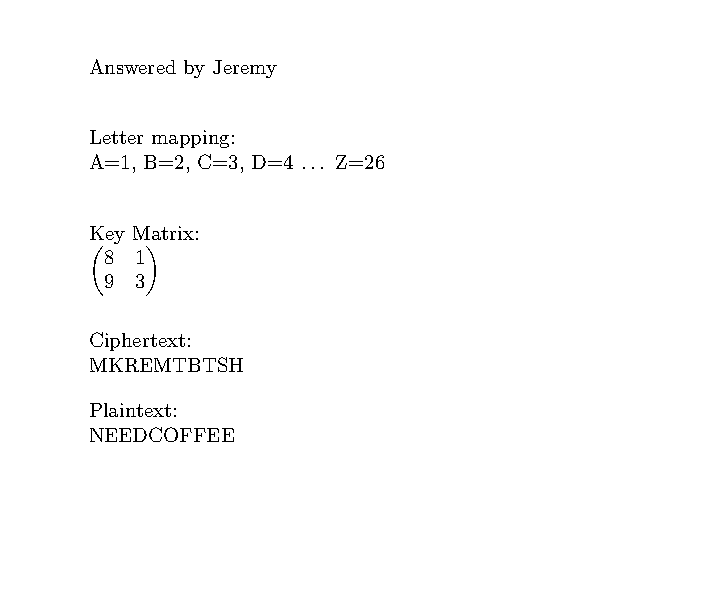
\includegraphics[width=0.5\linewidth]{Matrix_answer.pdf}
    \caption{Our answer sheet for the other student's ciphertext.}
    \label{fig:sheet}
\end{figure}

\subsection*{2. TI-84 Plus CE Calculator Workflow}

To verify these manual calculations using a TI-84 Plus CE graphing calculator:
\begin{enumerate}
    \item \textbf{Define Matrix A:} Press \texttt{[2nd]} $\rightarrow$ \texttt{[MATRIX]} $\rightarrow$ \texttt{EDIT} $\rightarrow$ select \texttt{[A]}, set size to $2\times2$, and input entries: $8, 1, 9, 3$.
    \item \textbf{Define Matrix B (Ciphertext Vector):} Set up matrix \texttt{[B]} as $2\times1$ with entries $13, 11$ (for block \texttt{MK}).
    \item \textbf{Calculate Determinant:} On the home screen, select \texttt{det([A])} to obtain \texttt{15}.
    \item \textbf{Verify GCD:} Press \texttt{[MATH]} $\rightarrow$ \texttt{NUM} $\rightarrow$ select \texttt{gcd(15, 26)}, which evaluates to \texttt{1}.
    \item \textbf{Perform Multiplication:} Compute \texttt{[C] * [B]} (where \texttt{[C]} is the inverse matrix $\smat{21&19\\15&4}$) to get $\vect{482\\239}$, then take each value modulo $26$ to find the plaintext vector.
\end{enumerate}

\section*{Appendix C: Program Output}

The saved output of \texttt{python hill\_toolkit.py all} is supplied as \texttt{sample\_output.txt} in the linked repository. It records the worked examples, counts, kernel test, fixed-block distribution and known-plaintext attacks. GPT ran the submitted version, and all five unit tests passed. With GPT support, the author interpreted the output and used the relevant results in the investigation. A later run in the local VS Code terminal also passed all five tests.


\clearpage
\section*{Appendix D: AI and Tool Use Disclosure}

\begin{itemize}
    \item \textbf{GPT (ChatGPT/Codex):} Generated and revised the Python code and tests, and ran the program checks. This included testing in the local VS Code terminal. The author used GPT explanations to understand the output, then used the coding results to develop the investigation. GPT also assisted with wording and revisions. It also assisted with the report structure, LaTeX and the refined-key investigation.
    \item \textbf{Writing Support (DeepL):} Used to refine academic phrasing and expression.
    \item \textbf{Learning Resources (YouTube \& Bilibili):} Utilized for researching and understanding mathematical concepts.
    \item \textbf{Typesetting (Overleaf):} Used for compiling and generating the final PDF document.
    \item \textbf{Calculations \& Verification:} Performed by hand, with modular reductions checked via CalculatorSoup and gcd values verified using a TI-84 Plus CE graphing calculator.
    \item \textbf{Programming and testing:} Completed by GPT using Python. The work covers encryption, decryption, key counting, fixed blocks, known-plaintext attacks and unit tests. It is not presented as code or tests independently produced by the author.
\end{itemize}



\end{document}
